\section{Background}
\label{sec:c2-background} % labe to enable hyperref to this chapter
\subsection{Private cars as a mode of transport in urban settings}
\justify

% Additional aspects this chapter could consider or dive in more deeply
%-- Donald Shoup's "The High Cost of Free Parking" (2011, revised edition)
%-- the space parked cars take
%-- amount of cars in urban settings
%-- interplay of parking policy, land use planning and urban settings, and adverse effects on environment (For example, \cite{Thompson1998}: Parker 1973, Gillen 1977, Feeney 1989)
%-- Benenson et al. research group is quite prolific, should look into it more
%-- additional PPGIS bibliography and map survey considerations

The number of private cars is globally on the rise. According to one estimation, the world reached one billion cars in 2020 (\cite{Sperling2009}). International Organization of Motor Vehicle Manufacturers (OICA) estimates that there were already at 950 million private cars in 2015 (\cite{OICA2020}). As the production of private cars is expected to continue, eyes must turn to managing the vast quantity of personal transportation in cities and in their surroundings. This is a question of mitigation of climate change, but also ensuring the economic performance of cities, and maximising the quality of life for urban citizens (\cite{Bertolini2003}).

Since the last century, urban landscapes have experienced change toward car based mobility, where streets have incrementally widened and parking standards continually increased. This space has been mostly taken from all other users of public space to accommodate cars (\cite{Cervero2017}). As cars have become a most common sight in cities, the mitigation of their adverse effects have become an important focus in policy. A major challenge cities face today is the relation of mobility of people and the urban land use. It has been shown that parking policy is an effective tool in the management of this challenge (\cite{Diallo2015}; \cite{Marsden2006}).

One goal of parking policy is an urban environment less dependant on private cars. However, a central issue in attempting to shape urban development in a direction that's less dependent on cars is that the alternatives fail to reach the quality of accessibility provided by private cars (\cite{Bertolini2003}). in \citeintext{Willson2013}, the author discusses that parking requirements have taken cities into a chokehold. The requirements are responsible of creating the most wasteful sections of transport and land use complexes, the unoccupied parking spaces. To alleviate this situation, Willson has developed a 12-step toolkit to help planners make more informed decisions on the subject. These steps include points such as accounting for market conditions, and the consideration for alternative modes of transport, such as shuttle services or bicycles. Results of this thesis aim to illustrate the actual parking conditions in Helsinki Capital Region, which could be of use to planners willing to take on Willson's toolkit.

\newpage
\subsection{Accessibility}
\justify

Considering transportation of people in cities, It may be thought that it is of highest priority to reach places as fast as possible. This is called \textit{spatial mobility}, movement which can be observed. However, people are ultimately not interested in measuring time units, but in social and economic interactions. It can then be said that the actual matter to focus in transporting people in cities is not mobility, but \textit{accessibility}. Accessibility can be defined as potential movement, observed through modelling. In accessibility, it is possible to attain a more realistic view into what is possible with available resources, such as time, and combine this with important issues regarding the sustainable development of cities. (\cite{Hodge1997}; \cite{Tenkanen2017}; \cite{Cervero2017})

First discussed by \citeauthor{Hansen1959} (\citeyear{Hansen1959}), accessibility as a concept has been widely studied in the decades that followed. In these first efforts, Hansen succeeded in showing that locations in Washington D.C., United States, that had good accessibility were more likely to end up developed. These areas would also be developed at a higher density.

Torsten Hägerstrand's classic time geography approach developed further the idea that accessibility is an intricate complex of interdisciplinary tendencies. Individuals can be viewed as a bearers of action spaces of varying sizes and durations, which are determined by their social role, income, and how advanced technology they can access. Individuals are bound to their time budgets which are indivisible from certain constraints: the capacity, coupling, and institutional constraints (\cite{Wegener1999}; \cite{Hagerstrand1970}).

Continuing on Hägerstrand's action-space line of thinking, Zahavi (\citeyear{Zahavi1974}) proposed that individuals are not attempting to minimise travel time or cost required for a number of activities, but to maximise what is available to them considering their travel times and monetary budgets. Zahavi's theory can explain why the expansion of private car use has been as extensive as it has been. According to \citeintext{Wegener1999}, the theory sheds light on why the motorisation in the twentieth century caused even longer and more car trips when travel speed gains were attained and why shopping centers in outskirts of cities can attract customers from ever more larger areas of influence. Moreover, indicated by the results of \citeintext{Salonen2014} and discussed in \citeintext{Jain2008}, it may be argued that individuals do not merely choose travel modes on economic terms, elaborating that travel time itself valuable. Individuals' travel time budget is explored in detail in \citeintext{Mokhtarian2004}.

More recently, \citeintext{Geurs2004} and \citeintext{Bertolini2003} have provided their definitions for accessibility. \citeauthor{Geurs2004} argue that accessibility should be associated with land use and transport systems in society and this would provide individuals with opportunities to take part in activities in different locations. According to \cite{Bertolini2003}, accessibility refers to the quantity and the diversity of spatial opportunities which can be reached within a certain amount of time.

\newpage
\subsection{Previous parking studies}
\justify

Parking is an important part of a traffic system as all vehicles need a storage location when they are not in use. Due to increasing amount of cars, cities being built on private car mobility, and parking policy trying to find a balance between raising activity locally and not deterring visitors, motorists have been shown to spend a large percentage of their overall travel chain \textit{searching for parking} (\cite{Axhausen1991}; \cite{Marsden2006}; \cite{Shoup2006}). A stressful experience for motorists, searching for parking has been identified as an eminent source of urban congestion (\cite{Axhausen1993}; \cite{Gantelet2006}), and parking policy improvements are much needed for most major cities (\cite{Benenson2008a}). According to \citeintext{Young1991}, the quantity and the location of parking affect:

\begin{itemize}
    \begin{singlespace}
        \item[--] the congestion on access roads and city streets;
        \item[--] the efficiency and financial performance of public transport;
        \item[--] comfort and safety levels of a city and the surroundings, and;
        \item[--] the form and functioning of the entire area.
    \end{singlespace}
\end{itemize}

As such, parking policy is closely interlocked with potential conflict within different levels of government, city residents, holders of commercial interest, and other special interest groups (\cite{Ker1988}). It does not help that parking policy is an urgent matter in most major cities: \citeintext{Arnott2006} states that on-street parking may be utilised to over 100 percent capacity due to double parking, illegal curbside parking, and parking on the sidewalk. One study found that motorists parking in unauthorised space in Paris, France, counts up to 62 percent of all parking events (\cite{Gantelet2006}). Inefficient parking policy also promotes \textit{cruising for parking}, a phenomenon which is partly a symptom of tension between demand and supply, and inefficiently low parking fees on-street (\cite{Shoup2004}; \citeyear{Shoup2006}). \citeintext{Martens2010} recognises three types of cruising for parking motorists: the commercial parkers, commuter parkers, and residential parkers.

Parking search problems originate from the mismatch between parking intentions of the motorists and available supply. In some more traditional cases, the mismatch can be addressed with expanding capacity or constrain demand, but in other cases the problem is spatially and temporally specific. For instance, that motorists' knowledge of local parking opportunities may be lacking, or road condition and layout is poor in specific places. (\cite{Axhausen1993})

In \citeintext{Teng2002}, off-street parking in New York, United States, was studied through a survey. Specifically pertaining to parking garages, the research quantified that increase in parking information markedly decreased parking search time. In their survey, the parking information most sought after by respondents were the fee structure, hours of operation, and the location on a map. The determinants of parking behaviour is further explored in \citeintext{Spitaels2008}, where both on-street and off-street parking locations are considered.

% tilde "~" indicates a non-breaking space
Based on the works of \citeintext{Layzell1985} and \citeintext{Polak1989}, \citeintext{Thompson1998} have defined the \textit{parking process} as a series of decisions by motorists based on updated knowledge gained from experience (figure~\ref{fig:parking-process-thompson}; a definition similar to this is also used by \citeintext{Guo2013}). The process commences on the start of searching for parking. Parking sites are examined and on the discovery of a favourable car park, a selection is made or the search continues (In \citeintext{Thompson1998} \textit{car park} means both off-street parking garages as well as on-street parking that share common attributes). After leaving a selected car park, the next leg of the parking search process begins. \citeauthor{Thompson1998} state that motorists must make a choice based on imperfect information, as aspects of the parking process are stochastic and opaque to individuals.

\begin{figure}[H]%
    \centering
    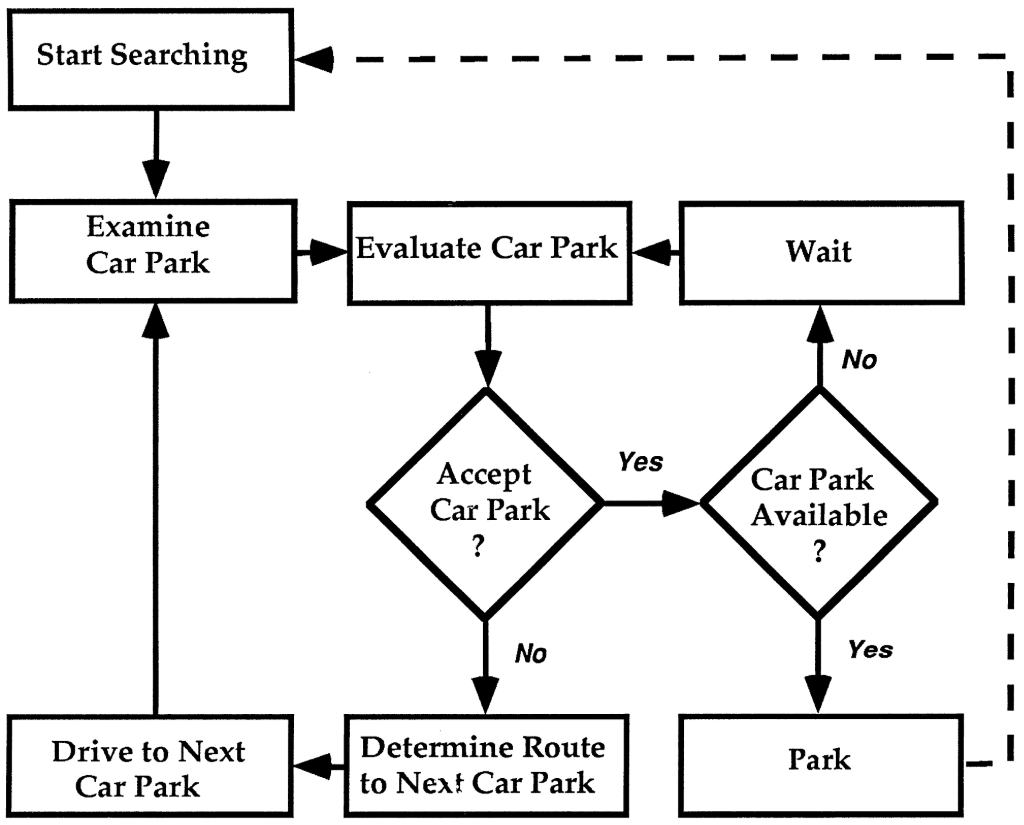
\includegraphics[width=.75\textwidth]{images/thesis_parking_search_process_thompson1998.PNG}
    \caption[Parking search process]{Defined by \citeauthor{Layzell1985} (\citeyear{Layzell1985}) and \citeauthor{Polak1989} (\citeyear{Polak1989}), parking choice may be considered as a search process in which motorists make linked decisions based on updated knowledge gained from experience. Figure adapted from \citeauthor{Thompson1998} (\citeyear{Thompson1998}).}%
    \label{fig:parking-process-thompson}%
\end{figure}

In \citeintext{Salonen2013}, the accessibility disparity is studied in a comprehensive manner. Many earlier accessibility studies are cast into doubt as they have been simplifying the subject matter, using methods that are not satisfactorily explained, or are simply incompatible. \citeauthor{Salonen2013} employ real data in finding compatible methods for calculating travel times for both private car and public transport. Introducing the \textit{door-to-door approach}, the researchers strove for maximum realism when calculating the duration of entire trips, or \textit{travel chains}. In the door-to-door approach for private car, all realistic parts of a journey are taken into account (figure~\ref{fig:door-to-door}). The trip starts at the point of origin (O), from where one walks to where their car is parked at (P). The car drive segment commences and continues until the earliest place where one would like to park at. This is where the parking process starts (see figure~\ref{fig:parking-process-thompson}), and it continues until a parking place is found and the car is parked (P). Finally one walks to the final destination of their journey (D). The door-to-door approach for the private car draws attention to a severely understudied subject, the parking process at the end of every trip made. While they accurately demonstrated the events that take place in realistic private car trips, \citeauthor{Salonen2013} themselves touched the subject of parking process only fleetingly. Notably, a parking process comparable to the one included in the door-to-door approach is described and employed in literature as early as in the 1960s (the "park-and-visit" approach, \cite{Inwood1966}; \cite{May1985}; \cite{Belloche2015}). 

\begin{figure}[H]%
    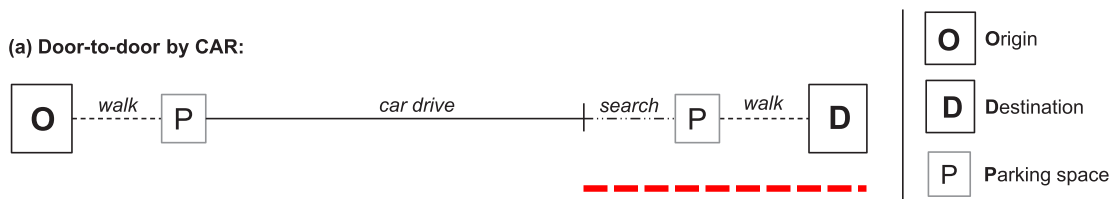
\includegraphics[width=\textwidth]{images/door2door.png}
    \caption[Door-to-door approach]{The entire travel chain of a private car using the door-to-door approach. The red dashed line represents the parking process segment of the travel chain. Figure adapted from \citeintext{Salonen2013}.}%
    \label{fig:door-to-door}%
\end{figure}

In this literary review to parking survey, it became apparent that most studies in this field employ a computational model to predict availability or use of parking spaces. Parking survey studies were sparse in number, and according to \citeintext{Diallo2015}, this is because the cost or difficulty to access appropriate data. They also note that complexity and extent of such studies work as a detriment.

In one computational model, \citeintext{VanDerGoot1982}, based on a parking study in the city of Haarlem, the Netherlands, showed that walking time strongly influenced drivers' choice of parking. An additional finding was that with the parking purpose of "shopping", longer walking times led to longer parking times, and shorter walking times translated to shorter parking times. In addition, in shopping trips, destination choice is influenced by the parking search time (\cite{Axhausen1993}). However, it is shown in literature that long term experience in parking search or knowledge of the area does not automatically result in better parking choices or make the parking search shorter (\cite{Thompson1998}; \cite{Teng2002}). \citeintext{Guo2013} has explored parking search process through an agent-based model in which a supply and demand are incorporated with sequential game-theorical capacity model to account for motorists' psychological attitudes in university campuses in the United States. 

\citeintext{Benenson2008} propose a parking process model that is spatially explicit and agent-based (termed "PARKAGENT"). This means that the model takes urban elements essential for investigating parking process into account and gives agents instructions on how to react in different circumstances, such as reactions to lack of parking spaces and parking enforcement efforts, to simulate parking behaviour of motorists. This paper shows that the addition of a new parking facility does not much improve average parking search time and walking distance for on-street parking motorists. This was because the new facility, essentially, would change the supply and demand scenario of that area, bringing in motorists to the area who have their journey destinations further away. The paper also states that traditional parking modelling is insufficient in saturated parking situations (most major cities), as it is not possible for these models to consider actions of independent agents who can make decisions on exact \acrfull{gis} data. A detailed view into "PARKAGENT" is described in \citeintext{Martens2010} alongside with a performance comparison to a non-spatial model of parking. A finding from this paper states that if parking turnover is low for a location (15 percent in an hour), the parking occupancy level of 85 percent, proposed by \citeintext{Shoup2004}, can be raised up to 95 percent. Parking occupancy level can be adjusted with changes to parking fees. The study also finds that if parking turnover reaches 50 percent for an hour, the aforementioned optimisation does not work.

Furthermore, \citeintext{Levy2015} propose the model termed "PARKFIT", an \acrshort{gis} algorithm for estimating parking patterns without the need for in-situ behavioural data, and a continuation for the research carried out on "PARKAGENT". If high-resolution infrastructure \acrshort{gis} layers are available, the algorithm can be used to produce estimations -- map views -- about average distances between private cars aiming for a specific destination and the actual destination parked at, and finally the proportion of cars that fail to find a parking place. The model, however, does not include parking search time.

In a commendably open, data-driven study, \citeintext{Aryandoust2019} provide methodology and tools for modelling car parking density maps using only travel time measurements. In the study, the freely available Uber travel time data is used to generate maps for 34 cities in multiple countries. \citeauthor{Aryandoust2019} manage to reach 90 percent accuracy for parking densities and 93 percent for circadian rhythm of the traffic in the chosen city of validation, Melbourne, Australia.

% \cite{Harris1997}: evaluate parking space availability at university campus 
% \cite{Saltzman1997}: on-street parking issues
Simulation to evaluate parking space availability has also been utilised in, for example, \citeintext{Harris1997} and \citeintext{Saltzman1997}.

\newpage
\subsection{Parking time estimations}
\justify

In accessibility studies, the estimations and measurements for parking times are relatively scarce and an understudied subject. In Finland, a parking survey research was conducted for the city of Tampere (\cite{Kalenoja2003}). The authors interviewed individuals that had just finished parking, and enquired after circumstances behind the parking, such as the factors that made them decide on the current parking place and from what direction they drove to the parking place location. In this study, 55 percent of interviewees had parked into a parking garage, 33 percent on-street and 13 percent in other areas. Over 60 percent of all interviewees reported that a short walking distance to their destination was of importance. The average time to find a parking place was 0.42 minutes on weekdays (table~\ref{tab:kalenoja-parktimes}).

\begin{hyphenrules}{nohyphenation}
    \begin{table}[H]
        \centering
        \caption[Parking time results in Kalenoja \& Häyrynen 2003]{The average time (minutes) to find a parking place in different types of locations in Tampere, Finland (\cite{Kalenoja2003}).} 
        \label{tab:kalenoja-parktimes}
        \begin{tabular}{ llll }
            \toprule
            Parking place type  & Weekday   & Saturday  & Overall \\
            \midrule
            On-street           & 0.73      & 2.08      & 0.80 \\
            Other areas         & 0.16      & 0.38      & 0.18 \\
            Parking garages     & 0.22      & 0.55      & 0.33 \\
            Overall             & 0.42      & 0.65      & 0.46 \\
            \bottomrule
        \end{tabular}
    \end{table}
\end{hyphenrules}

Internationally, \citeintext{Shoup2006} has been a landmark paper in private car parking time research. Mustering all research there was available on \textit{cruising for parking}, Shoup was able to display a compilation of results from a wide temporal and spatial pool. The gathered data showed that a range of 8--74 percent of a total trip was spent in cruising for parking. The average time to find a curbside parking place was in the range of 3.5--14 minutes. Shoup himself acknowledges the wide variance, saying that in reality some cities may have zero time spent in cruising for parking, while in other locations a large portion of a journey made with private car consists of it. Regarding time spent in searching for parking when traveling by private car, \citeintext{Polak1990} state that it may constitute up to 25 percent of the average total travel time. According to \citeintext{Axhausen1991}, motorists value short parking search times over the driving time, with parking search time being up to two times more valuable. \citeintext{Parmar2020} suggest, based on their literature review, that motorists prefer to minimise the "out-vehicle" costs of parking charges, cruising for parking, and walking times, rather than the costs pertaining to the car itself, such as fuel cost and driving time.

In a parking time research carried out in France, it was found out that the average parking search time was especially severe in Paris. In the districts studied in Paris, parking search lasted on average 10 minutes in Commerce district and 7.7 minutes in Saint-Germain district. Extrapolating their results to the entire France, the researchers estimated that 70 million hours, each year, is spent searching for parking places (\cite{Gantelet2006}). In an other parking time focused paper, on-street parking was modelled and validated with a parking survey. The survey, conducted in Lyon, France, showed especially intolerable parking times in districts near the center of Lyon: an average searching time of 11.1 minutes for Part-Dieu, 9.6 minutes for Charpennes, and 6.3 minutes for Belges. All of these districts provided parking free of charge. In this study, the longest average parking search duration for a district with parking meters was the center of Lyon, Presqu'île, with a result of 6.2 minutes (\cite{Belloche2015}).

\newpage
\subsection{Research in participatory GIS and map surveys}
\justify

In \citeintext{Salonen2014}, \acrfull{ppgis} was employed in understanding what is the character of daily mobility in the Helsinki Capital Region and how often the fastest travel mode (in this study, "the most optimal") is selected in these everyday trips. The data received from respondents was compared to routes calculated with advanced multimodal routing models presented in \citeintext{Salonen2013}. The study found that respondents most often chose non-optimal travel modes on "bounded trips" (work, school, or day care) and that instead of the private car, many of the respondents are ready to choose a slower, and less carbon emission intensive means of travel.

\citeintext{Laatikainen2015} made use of \acrshort{ppgis} in the context of accessibility to urban aquatic environments and the environmental justice perspective that is included in a premise such as this. Employing "SoftGIS" methodology, the researchers were able to gather a large amount of data from users of urban environments through an easy-to-use user interface on the internet (\cite{Kytta2011}). The researchers had the opportunity to make use of Finnish Population Register to select a group of potential respondents representative of the study area, the Helsinki Capital Region. In some of the results, researchers point out that even though water is almost omnipresent in the Helsinki Capital Region, the utilisation of \acrshort{ppgis} revealed that proximity of a body of water does not have a clear influence on the real usage, or travel distances and times. This being said, the results showed that in many cases the body of water nearest to an individual was undesirable in some way, prompting the individuals to seek amenities along waterside further away. Also, while some areas of the Helsinki Capital Region are closer to more bodies of water, this fact did not automatically mean good access because of matters such as land ownership issues.

This thesis employs \acrshort{ppgis} in its parking research, approaching the subject matter with a \textit{do-it-yourself} mentality. While \citeintext{Salonen2014} expected low response rate for their survey research, this thesis aims to demonstrate that extensive scientific data can be feasibly collected in a public participation arrangement with minimal resources, making use of free and open source software in the system design and social media platform communities in the collection of the data.